%%%%%%%%%%%%%%%%%%%%%%%%%%%%%%%%%%%%%%%%%
% a0poster Landscape Poster
% LaTeX Template
% Version 1.0 (22/06/13)
%
% The a0poster class was created by:
% Gerlinde Kettl and Matthias Weiser (tex@kettl.de)
% 
% This template has been downloaded from:
% http://www.LaTeXTemplates.com
%
% License:
% CC BY-NC-SA 3.0 (http://creativecommons.org/licenses/by-nc-sa/3.0/)
%
%%%%%%%%%%%%%%%%%%%%%%%%%%%%%%%%%%%%%%%%%

%----------------------------------------------------------------------------------------
%	PACKAGES AND OTHER DOCUMENT CONFIGURATIONS
%----------------------------------------------------------------------------------------

\documentclass[a0,landscape]{a0poster}

\usepackage{multicol} % This is so we can have multiple columns of text side-by-side
\columnsep=100pt % This is the amount of white space between the columns in the poster
\columnseprule=3pt % This is the thickness of the black line between the columns in the poster

\usepackage[svgnames]{xcolor} % Specify colors by their 'svgnames', for a full list of all colors available see here: http://www.latextemplates.com/svgnames-colors

\usepackage{pgfpages}
\pgfpagesdeclarelayout{resize and center}
{
  \def\pgfpageoptionborder{0pt}
}
{
  \pgfpagesphysicalpageoptions
  {%
    logical pages=1,%
    physical height=\pgfpageoptionheight,%
    physical width=\pgfpageoptionwidth%
  }
  \pgfpageslogicalpageoptions{1}
  {%
    resized width=\pgfphysicalwidth,%
    resized height=\pgfphysicalheight,%
    border shrink=\pgfpageoptionborder,%
    center=\pgfpoint{.5215\pgfphysicalwidth}{.47\pgfphysicalheight}%
  }%
}
\pgfpagesuselayout{resize and center}[a2paper,landscape]

\usepackage{times} % Use the times font
%\usepackage{palatino} % Uncomment to use the Palatino font

\usepackage{graphicx} % Required for including images
\graphicspath{{figures/}} % Location of the graphics files
\usepackage{booktabs} % Top and bottom rules for table
\usepackage[font=small,labelfont=bf]{caption} % Required for specifying captions to tables and figures
\usepackage{amsfonts, amsmath, amsthm, amssymb} % For math fonts, symbols and environments
\usepackage{wrapfig} % Allows wrapping text around tables and figures
\usepackage[none]{hyphenat}

\begin{document}

%----------------------------------------------------------------------------------------
%	POSTER HEADER 
%----------------------------------------------------------------------------------------

% The header is divided into three boxes:
% The first is 55% wide and houses the title, subtitle, names and university/organization
% The second is 25% wide and houses contact information
% The third is 19% wide and houses a logo for your university/organization or a photo of you
% The widths of these boxes can be easily edited to accommodate your content as you see fit

\begin{minipage}[b]{0.55\linewidth}
\veryHuge \color{DarkOrange} \textbf{Location Sensitive Social Notifier} \color{Black}\\ % Title
\Huge\textit{Location based, messaging platform for Android smartphones}\\[1cm] % Subtitle
\huge \textbf{Thomas Mark Rosier}\\ % Author(s)
\huge Aberystwyth University, Computer Science Department\\ % University/organization
\end{minipage}
%
\begin{minipage}[b]{0.25\linewidth}
\color{DarkSlateGray}\Large \textbf{Contact Information:}\\
Department of Computer Science\\
Llandinam Building\\
Aberystwyth University\\
Aberystwyth\\
Ceredigion\\
SY23 3DB\\ 
Email: \texttt{thr2@aber.ac.uk}\\ % Email address
\end{minipage}
%
\begin{minipage}[b]{0.19\linewidth}
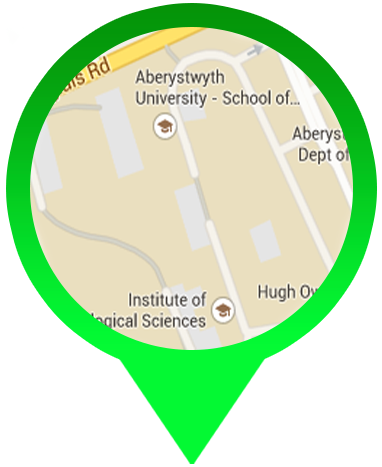
\includegraphics[width=12cm]{logo.png} % Logo or a photo of you, adjust its dimensions here
\end{minipage}

\vspace{1cm} % A bit of extra whitespace between the header and poster content

%----------------------------------------------------------------------------------------

\begin{multicols}{4} % This is how many columns your poster will be broken into, a poster with many figures may benefit from less columns whereas a text-heavy poster benefits from more

\color{Navy}
\section{Abstract}

\color{Olive}
\section{Introduction}

\color{Black}
\section{Aims of the project}

Aims of location sensitive social notifier is to give users the ability to post tags onto specific locations and theses tags to be able to be picked up by there followers, this functionality is given to the users through the use of an Android application with a simple and intuitive user interface to allow them to easily post messages.\\
\\
For users that have the application installed one of the main aims of the application was to make it so that the users can easily pick up notifications and to also preserve power on the users device so that running the application does not drain the phones battery while trying to seek out users relevant tags.\\
\\
The concept of the application has be carried out before but using hardware tags as a focal point, so a user would add a bluetooth tag to a physical location and the phone would pick this up and deliver a message to the user, the goal of the project was to try and achieve this functionality without the use of a hardware device and just using the services provided by modern Android smartphones most notability GPS positioning to get the tags to the end user.

\section{Progress so far}

Development of the application has reached a proof of concept stage of development, where users can generate messages for other users to view, and are picked up on the other users devices when they have entered a reasonable proximity to the message. The application has been developed in a eXtream Programming approach which means that the functionality of the application has only been implemented as it has been needed, this has been used in conjunction with a Test Driven Development approach which means that each bit of functionality within the application is robustly tested and when new functionality is added to the application that the new functionality does not break the application.\\
\\
The Android side of the application is very much a work in progress with very few of the components fully completed it has skeleton of the application to show the concept works, The server side part of the application is reaching maturity with the most of the functionality implemented where it has been needed with the underlying structure completed for the future functionality that will be added to the application, the design and implementation of the database is almost complete and with minor tweaks that will need to be applied as development proceeds, optimisation will need to be carried out on all levels of the application to ensure that the application is efficient and quick to use, consideration has been taken to this point but has yet to be implemented.

\section{Technical details}

Lo Se Sono is primarily an Android project but it does us a number of other technologies to make it work effectively, Additional technology that is used along side the standard Google Android SDK is the Google Maps API for Android this extra API enables the use of mapping within the application, and is the main API that is hooked into the application everything else within the application is either from the standard Android SDK or bespoke.\\ 
\\
The location detection is carried out by the standard GPS package provided by the Android SDK and has been built up to enable more support for using GPRS data along side the use of GPS, the calculations algorithm for the distance was based off work by Chris Veness in the paper (Calculate distance, bearing and more between Latitude/Longitude points).\\
\\
The backend of the application uses the Node.JS runtime which is based of the Google Javascript engine, this is used in conjunction with HAPI.JS to provide a REST interface for the android application to interact with, HAPI provides its own security API's to interact with providing basic authentication for the application along with a primitive cookie based application system to give authentication to the end user. The Node/HAPI application provides a connecting piece between the Android application and the database, most of the processing and computation is carried out within the database engine.\\
\\
The database technology that has been used is PostgresSQL, this was chosen as it provides much more flexibility and extended functions over SQLite or MySQL, the application takes advantaged of the extensive JSON support provided by PostGresSQL along with the advanced Database functions to do fast processing within the database engine rather than context switching back to the Node application to carry out the work which in turn should make the application more responsive and should speed up processing. All of the authentication is handled within the database with the storing of user credentials and the hashing of the user passwords to ensure that they are stored safely, PostGresSQL provides all the hashing and encryption packages that are needed to ensure that sensitive data is stored safely.

\section{Future development}

One of the major features that will be added later on development, will the ability to hook into the Facebook infrastructure, to discover friends and to share notification on their platform rather than being isolated from the greater social networking force, having Facebook infrastructure within should greatly improve adoption of the application and also easing the use of the application and adding users friends to the application.\\
\\
There is also the possibility of the development of a companion Pebble smartwatch application that will give the user the ability to quickly tag a location from there wrist with a list of pre-defined messages, this is an interesting nice to have and will help the penetration of the market with interesting ideas and help with the adoption of smart watches.\\
\\
If the application proves successful it is very likely that a iOS version of the application will be developed for Apple iPhones, this should help with the popularity of the application and should ensure that their is a much greater market coverage for the service.

\section{Acknowledgments}

Cian O'Shaughnessy - Graphics\\
Chris Veness - GPS distance calculation algorithm\\

%----------------------------------------------------------------------------------------

\end{multicols}
\end{document}